\let\textcircled=\pgftextcircled
\chapter{Introduction}
\label{chap:intro}

Begins a chapter.

%=======
\section{Section}
\label{sec:sec01}

Begins a section.

Acronym examples This one is about \acrlong{gcm} (\acrshort{gcm}). This is best done with \acrfull{cpm}.

\subsection{Subsection}
\label{subsec:subsec01}

Begins a subsection.

% A single figure
\begin{figure}[t!]
	\centering
	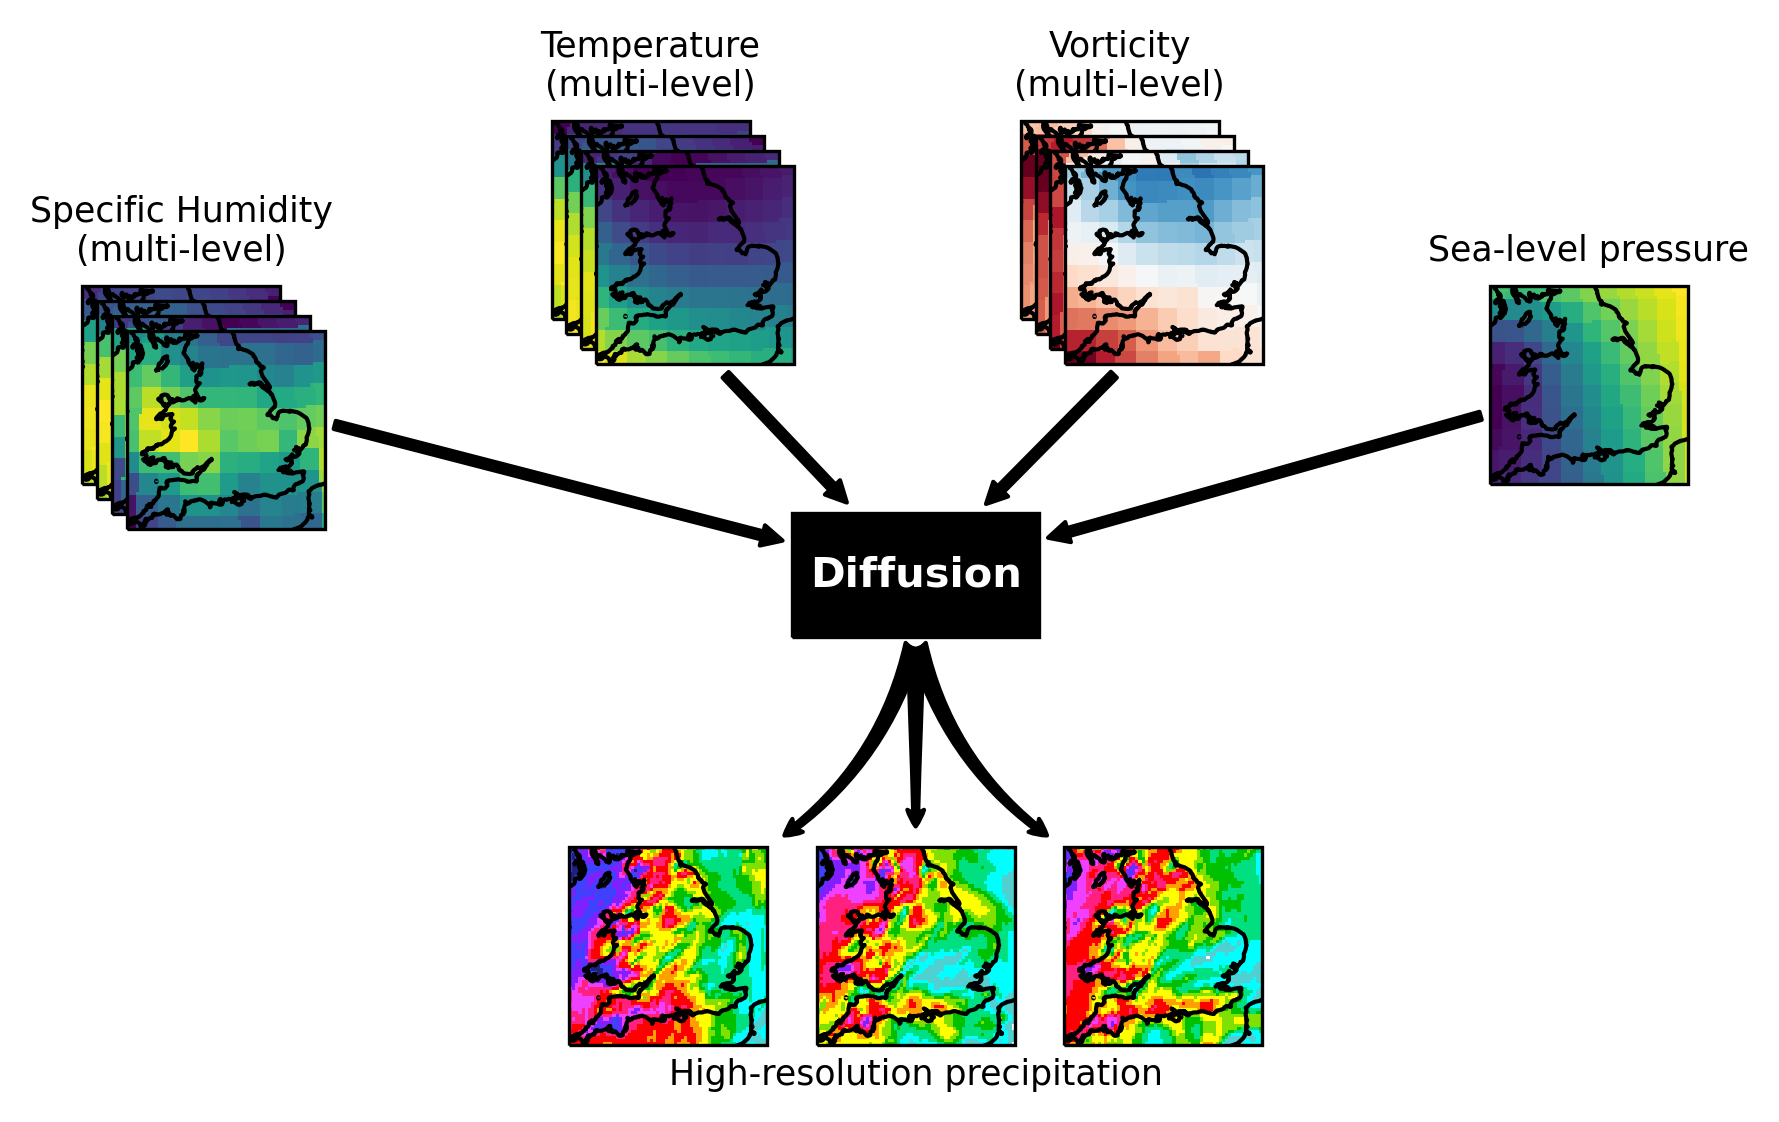
\includegraphics[height=0.35\textheight]{chapters/fig01/ai-schematic.png}
	\caption{CPM precip emulator schematic. Figure reproduced from \cite{Addison2024diffcpmprecipemul}.}
	\label{fig:RHP02}
\end{figure}
